\chapter{Basic data structures}

This chapter uses Big-O notation when discussing the performance of various data structures for different tasks, see the Asymptotics chapter for this.

\section{Arrays}

\begin{definition}
    A sequence of \textbf{elements} $a_0, a_1, \ldots, a_{n-1}$ is called an \textbf{array} of size $n$. We usually denote arrays as 
    \begin{center}
        \texttt{A[0], A[1], ..., A[n-1]} \quad or \quad \texttt{A[0...n-1]}
    \end{center}
    An array is such that the memory addresses of each element can be computed from the memory location of the first element and the index of the element. The simplest type of this data structure is a \textbf{linear array}. They are stored in consecutive memory cells. The size of an array must be specified when it is defined and cannot be changed.
\end{definition}

\begin{remark}
    Typically the data type of all the elements in an array is the same, however, some implementations of arrays in programming languages do not follow this.
\end{remark}

\begin{example}
    Say we have an array of four $16$-bit integer variables with indices $0$ through $3$. This may be stored at memory addresses $1000$, $1002$, $1004$, and $1006$, so that each element with index $i$ has the address $1000+2i$.
\end{example}

\begin{figure}
    \centering
    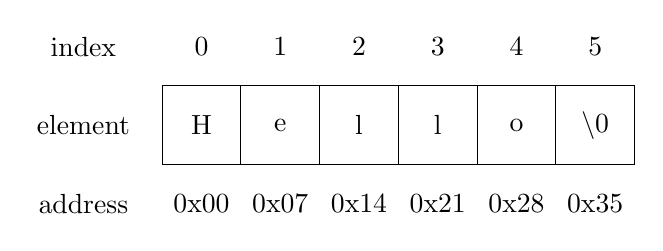
\begin{tikzpicture}
        \draw (0.5,1.5) node {0};
        \draw (1.5,1.5) node {1};
        \draw (2.5,1.5) node {2};
        \draw (3.5,1.5) node {3};
        \draw (4.5,1.5) node {4};
        \draw (5.5,1.5) node {5};
        \draw (0,0) rectangle node {H} (1,1);
        \draw (1,0) rectangle node {e} (2,1);
        \draw (2,0) rectangle node {l} (3,1);
        \draw (3,0) rectangle node {l} (4,1);
        \draw (4,0) rectangle node {o} (5,1);
        \draw (5,0) rectangle node {\textbackslash0} (6,1);
        \draw (0.5, -0.5) node {0x00};
        \draw (1.5, -0.5) node {0x07};
        \draw (2.5, -0.5) node {0x14};
        \draw (3.5, -0.5) node {0x21};
        \draw (4.5, -0.5) node {0x28};
        \draw (5.5, -0.5) node {0x35};
        \draw (-1, 1.5) node {index};
        \draw (-1, 0.5) node {element};
        \draw (-1, -0.5) node {address};
    \end{tikzpicture}
    \label{fig:hello_string}
    \caption{Visualisation of the array data structure.}
\end{figure}

\begin{example}
    Say we want to store the string \texttt{Hello} as an array of characters where each character requires $7$-bits. We will need the array to be of size $6$ for the $5$ characters and the necessary escape character to represent the end of the string. Figure \ref{fig:hello_string} shows how the characters would be stored.
\end{example}

\begin{remark}
    In the last example the notation \texttt{0x00} was used to represent a memory address. The prefix \texttt{0x} tells us that the number afterwards is a hexadecimal number, this is commonly used to represent values stored on the computer.
\end{remark}

\subsection{Performance}

The main benefit of using arrays is that they have $O(1)$ indexing and have no wasted space since all data is stored consecutively. As arrays have fixed size you cannot allocate or deallocate memory (unless you deallocate the memory for the last element), therefore, to insert or delete elements (and their allocated space) you would have to redefine a new array and move the elements back in which is not efficient.

\section{Lists}

\begin{definition}
    A \textbf{linked list} is made up of \textbf{nodes}. Each node stores an \textbf{element} and a \textbf{pointer} to another node. The first node is called the \textbf{head} and the last node is called the \textbf{tail} which has a null pointer. This data structure can be scattered over memory; it does not have to be stored consecutively.
    
    For linked list $L$, we may use the following notation:
    \begin{enumerate}[label=(\roman*)]
        \item \texttt{L.head}, the pointer for the head of the list and
        \item \texttt{L.tail}, the pointer for the tail of the list.
    \end{enumerate}
    For node $N$ we may use the following notation:
    \begin{enumerate}[label=(\roman*)]
        \item \texttt{N.data}, the element;
        \item \texttt{N.next}, the pointer to the next node in the list (or \texttt{NULL} if at the tail).
    \end{enumerate}
\end{definition}

\begin{definition}
    A \textbf{null pointer}, written \texttt{NULL}, represents an undefined value.
\end{definition}

\subsection{Performance}

Indexing a linked list has average time complexity $O(n)$ as we have to traverse every node prior to the node, making it quite inefficient in this regard; however, linked lists allow us to be \emph{dynamic} with the size of the data structure. Linked lists allow efficient insertion and deletion; inserting and deleting elements from a linked list has time complexity $O(1)$.

\subsection{Implementation}

We can implement a singly linked list in C++ using the following listings, as shown in Listings \ref{lst:singly_node_struct}, \ref{lst:singly_data_struct}, \ref{lst:singly_find}, \ref{lst:singly_insert}, and \ref{lst:singly_delete}.

\begin{lstlisting}[float,
                  language = C++,
                  caption = {Node data structure for singly linked list in C++.},
                  label = lst:singly_node_struct]
class Node {
public:
    Node *next = nullptr;
    int data;
};
\end{lstlisting}

\begin{lstlisting}[float,
                  language = C++,
                  caption = {Singly linked list data structure in C++.},
                  label = lst:singly_data_struct]
class LinkedList {
public:
    Node *head = nullptr;
    Node *tail = nullptr;
    int size = 0;

    LinkedList() = default;

    // other functions...
};
\end{lstlisting}

\begin{lstlisting}[float,
                  language = C++,
                  caption = {Find function for singly linked list in C++.},
                  label = lst:singly_find]
int Find(int data) {
    Node *temp = head;
    for (int i = 0; i < size; ++i) {
        if (temp->data == data) {
            return i;
        }
        temp = temp->next;
    }
    return -1;
}
\end{lstlisting}

\begin{lstlisting}[float,
                  language = C++,
                  caption = {Insert function for singly linked list in C++.},
                  label = lst:singly_insert]
void Insert(int data) {
    Node *temp = new Node();
    temp->data = data;
    temp->next = head;
    head = temp;
    size++;
}     
\end{lstlisting}

\begin{lstlisting}[float,
                  language = C++,
                  caption = {Delete function for singly linked list in C++.},
                  label = lst:singly_delete]
void Delete(int data) {
    if (head->data == data) {
        head = head->next;
        size--;
    } else {
        Node *node = head->next;
        Node *prev = head->next;
        for (int i = 1; i < size; ++i) {
            if (node->data == data) {
                prev->next = node->next;
                size--;
                return;
            }
            prev = node;
            node = node->next;
        }
    }
}     
\end{lstlisting}

\subsection{Doubly linked list}

\begin{definition}
    \textbf{Doubly linked list} are an extension of what we have just defined (singly linked lists); a node in a \textbf{doubly} linked list stores two references:
    \begin{enumerate}[label=(\roman*)]
        \item a pointer to the next node in the list and
        \item a pointer to the previous node in the list.
    \end{enumerate}
\end{definition}

Typically, we place sentinel nodes at the head \texttt{L.head} and tail \texttt{L.tail} such that \texttt{L.head.prev = NULL} and \texttt{L.tail.next = NULL} but so that \texttt{L.head.next} and \texttt{L.tail.prev} are valid pointers. A doubly linked lists the head and tail sentinel nodes immediately accessible; therefore, traversal of the list can be done from the beginning or the end. Any node of a doubly linked list can be used to traverse the entire list. The size of a doubly linked list may also be stored.

The only difference in performance for a doubly linked list is that on insertion or deletion of an element, $2$ pointers will have to be updated instead of $1$ pointer for singly linked list.

The implementation in C++ is a bit more complicated as we need to update both pointers when inserting and removing nodes, as shown in Listings \ref{lst:doubly_node_struct}, \ref{lst:doubly_insert_front}, \ref{lst:doubly_insert_back}, and \ref{lst:doubly_delete}. The implementation for the find function remains the same. 

\begin{lstlisting}[float,
                  language = C++,
                  caption = {Data structure for node in doubly linked list in C++.},
                  label = {lst:doubly_node_struct}]
class Node {
public:
    Node *next = nullptr;
    Node *prev = nullptr;
    int data;
};
\end{lstlisting}

\begin{lstlisting}[float,
                  language = C++,
                  caption = {Insert to the head function for doubly linked list in C++.},
                  label = {lst:doubly_insert_front}]
void InsertFront(int data) {
    Node *temp = new Node();
    temp->data = data;
    if (size == 0) {
        head = temp;
        tail = temp;
    } else {
        temp->data = data;
        temp->next = head;
        temp->next->prev = temp;
        head = temp;
    }
    size++;
}
\end{lstlisting}

\begin{lstlisting}[float,
                  language = C++,
                  caption = {Insert to the tail function for doubly linked list in C++.},
                  label = {lst:doubly_insert_back}]
void InsertBack(int data) {
    Node *temp = new Node();
    temp->data = data;
    if (size == 0) {
        head = temp;
        tail = temp;
    } else {
        temp->data = data;
        temp->prev = tail;
        temp->prev->next = temp;
        tail = temp;
    }
    size++;
}
\end{lstlisting}

\begin{lstlisting}[float,
                  language = C++,
                  caption = {Delete function for for doubly linked list in C++.},
                  label = {lst:doubly_delete}]
void Delete(int data) {
    if (size == 0) {
        return;
    }
    if (head->data == data) {
        head = head->next;
        head->prev = nullptr;
        size--;
    } else {
        Node *node = head->next;
        for (int i = 1; i < size; ++i) {
            if (node->data == data) {
                node->prev->next = node->next;
                node->prev = node->prev;
                size--;
                return;
            }
            node = node->next;
        }
    }
}
\end{lstlisting}

\subsection{Circularly linked lists}

\begin{definition}
    \textbf{Circularly linked lists} are also an extension of singly linked lists, nodes are also defined the same as in singly linked list, that is, each node has a next pointer and the data it is holding. However, there is no beginning or end, such that where normally the last element in a singly linked list would point to \texttt{null}, instead, it points to the first node in the list. As there is no beginning or end, we mark a node on the list as the \textbf{cursor} which is the starting node when we traverse the list.
\end{definition}

Performance of a circularly linked list is similar to a singly linked list, benefits come from problems that have a circular nature to them and that you can traverse the entire list from any given node. 

Implementation again changes a little compared to singly or doubly linked lists, as shown in Listings \ref{lst:circularly_data_structure}, \ref{lst:circularly_insert}, and \ref{lst:circularly_delete}.

\begin{lstlisting}[float,
                  language = C++,
                  caption = {Circularly linked list data structure in C++.},
                  label = lst:circularly_data_structure]
class CircularlyLinkedList {
public:
    Node *cursor = nullptr;
    int size = 0;

    // other functions...
}
\end{lstlisting}

\begin{lstlisting}[float,
                  language = C++,
                  caption = {Insert function for circularly linked list data structure in C++.},
                  label = lst:circularly_insert]
void Insert(int data) {
    Node *node = new Node();
    node->data = data;
    if (size == 0) {
        node->next = node;
        cursor = node;
    } else {
        node->next = cursor->next;
        cursor->next = node;
    }
    size++;
}
\end{lstlisting}

\begin{lstlisting}[float,
                  language = C++,
                  caption = {Delete function for circularly linked list data structure in C++.},
                  label = lst:circularly_delete]
void Delete(int data) {
    if (size == 0) {
        return;
    }
    if (size == 1 && cursor->data == data) {
        cursor = nullptr;
    } else {
        Node *node = cursor->next;
        Node *prev = cursor;
        for (int i = 1; i < size; ++i) {
            if (node->data == data) {
                prev->next = node->next;
                return;
            }
            prev = node;
            node = node->next;
        }
    }
    size--;
}
\end{lstlisting}

\section{Stacks}

\begin{definition}
    A \textbf{stack} is a collection of objects that are inserted and removed according to the \textbf{last-in-first-out} (LIFO) principle.
    
    Objects can be inserted to the stack at any time, but only the most recently inserted objected can be removed at any time. Or more formally, a stack must have the methods
    
    \begin{enumerate}
        \item \texttt{push(e)}, insert element \texttt{e} at the top of the stack and
        \item \texttt{pop()}, remove and return the top element of the stack.
    \end{enumerate}
    
    Other miscellaneous methods are
    \begin{enumerate}[resume]
        \item \texttt{size}, return the number of elements in the stack;
        \item \texttt{IsEmpty}, return boolean values indicating whether or not the stack is empty (though this seems to be pointless giving that it is equivalent to \texttt{size == 0}); and
        \item \texttt{top}, return the top element of the stack without removing it.
    \end{enumerate}
\end{definition}

\begin{example}
    Given an initially empty stack $S$, what is the contents of $S$ after the following methods are called and specify any exceptions thrown:
    \begin{center}
        \texttt{S.push(5)}, \quad \texttt{S.push(3)}, \quad \texttt{pop()}, \quad \texttt{push(7)}, \quad \texttt{pop()}, \quad \texttt{top()}, \quad \texttt{pop()}, \quad \texttt{pop()}.
    \end{center}
    
    The stack will be empty after these functions are executed and there will be an \texttt{EmptyStackException} thrown on the last function call as it will be empty before the function is called.
\end{example}

The implementation for a stack in C++ is shown in Listings \ref{lst:stack_data_type}, \ref{lst:stack_push}, \ref{lst:stack_pop}, \ref{lst:stack_get_top}, and \ref{lst:stack_get_size}.

\begin{lstlisting}[float,
                  language = C++,
                  caption = {Stack data type in C++.},
                  label = {lst:stack_data_type}]
#define MAX_SIZE 32
class Stack {
private:
    int data_array[MAX_SIZE] = {};
    int size = 0;
public:
    Stack () = default;
    // other functions
};
\end{lstlisting}

\begin{lstlisting}[float,
                  language = C++,
                  caption = {Push function for stack data type in C++.},
                  label = {lst:stack_push}]
void Push(int data) {
    if (size == MAX_SIZE) {
        return;
    }
    data_array[size] = data;
    size++;
}
\end{lstlisting}

\begin{lstlisting}[float,
                  language = C++,
                  caption = {Pop function for stack data type in C++.},
                  label = {lst:stack_pop}]
int Pop() {
    if (size == 0) {
        std::cerr << "Stack empty." << std::endl;
        return -1;
    }
    size--;
    return data_array[size];
}
\end{lstlisting}

\begin{lstlisting}[float,
                  language = C++,
                  caption = {Get top element function for stack data type in C++.},
                  label = {lst:stack_get_top}]
int get_top() {
    if (size == 0) {
        std::cerr << "Stack empty." << std::endl;
    }
    return data_array[size - 1];
}
\end{lstlisting}

\begin{lstlisting}[float,
                  language = C++,
                  caption = {Get size function for stack data type in C++.},
                  label = {lst:stack_get_size}]
int get_size() {
    return size;
}
\end{lstlisting}

This implementation with arrays is time efficient as all methods are $O(1)$; however, the stack has a fixed maximum size due to being implemented with arrays. If the size of the stack is much less that this fixed maximum then we waste the allocated memory that is not used. Additionally, if the size of the stack exceeds the maximum size we will generate an exception. A linked list implementation of a stack would get around this.

% todo implement linked list stack

\section{Queues}

\begin{definition}
    A \textbf{queue} is a collection of objects that are inserted and removed according to the \textbf{first-in-first-out} (FIFO) principle. Element access and deletion are restricted to the first element in the sequence, called the \textbf{front} of the queue. Element insertion is restricted to the end of the sequence, which is called the \textbf{rear} of the queue.
    
    A queue supports the methods
    
    \begin{enumerate}
        \item \texttt{enqueue(e)}, insert element \texttt{e} at the rear of the queue;
        \item \texttt{dequeue()}, remove and return from the queue the element at the front;
    \end{enumerate}
    and possibly
    
    \begin{enumerate}[resume]
        \item \texttt{size};
        \item \texttt{isEmpty}, although this is equivalent to \texttt{size == 0}; and
        \item \texttt{front}.
    \end{enumerate}
\end{definition}

\begin{example}
    Queue examples
enqueue(5)
enqueue(3)
dequeue
enqueue(7)
dequeue
front
dequeue
dequeue
isEmpty
\end{example}

Let $A[1\ldots n]$ be an array of size $n$, $f$ be the index corresponding to the front of the queue, and $r$ be the index corresponding to the end of the queue. Initially, we assign $f=r=0$ saying that the queue is empty. Every time the \textbf{enqueue} method is called, we increment $r$, and every time the \textbf{dequeue} method is called, we increment $f$. To avoid an \emph{array out of bounds} error, we wrap around the end of $A$ by using
\[A[i\bmod n].\] Listings \ref{lst:queue_data_type}, \ref{lst:queue_queue}, \ref{lst:queue_enqueue}, \ref{lst:queue_get_top}, and \ref{lst:queue_get_size} shows an implementation of queues in C++ using arrays that uses this wrap around method to avoid array out of bounds errors.

\begin{lstlisting}[float,
                  language = C++,
                  caption = {Queue data type in C++.},
                  label = {lst:queue_data_type}]
#define MAX_SIZE 32

class QueueWithArray {
private:
    int data_array[MAX_SIZE] = {};
    int size = 0;
    int front_index = 0;
    int rear_index = 0;
public:
    QueueWithArray() = default;
    // other functions
};
\end{lstlisting}

\begin{lstlisting}[float,
                  language = C++,
                  caption = {Queue function for queue data type in C++.},
                  label = {lst:queue_queue}]
void QueueItem(int data) {
    if (size == MAX_SIZE) {
        std::cerr << "Stack full." << std::endl;
        return;
    }
    if (size == 0) {
        data_array[front_index] = data;
    } else {
        rear_index = (rear_index + 1) % MAX_SIZE;
        data_array[rear_index] = data;
    }
    size++;
}
\end{lstlisting}

\begin{lstlisting}[float,
                  language = C++,
                  caption = {Enqueue function for queue data type in C++.},
                  label = {lst:queue_enqueue}]
int Enqueue() {
    if (size == 0) {
        std::cerr << "Stack empty." << std::endl;
        return -1;
    }
    front_index = (front_index + 1) % MAX_SIZE;
    size--;
}
\end{lstlisting}

\begin{lstlisting}[float,
                  language = C++,
                  caption = {Front top element function for queue data type in C++.},
                  label = {lst:queue_get_top}]
int Front() {
    return data_array[front_index];
}
\end{lstlisting}

\begin{lstlisting}[float,
                  language = C++,
                  caption = {Get size function for queue data type in C++.},
                  label = {lst:queue_get_size}]
int get_size() {
    return size;
}
\end{lstlisting}

% can you use linked lists to implement queues

\section{Hash tables}

\begin{definition}
	A \textbf{hash function} $h$ is any function that can be used to map data of arbitrary size to data of a fixed size. The values returned by the hashes are called \textbf{hash values} (or \textbf{hashes}).
\end{definition}

\begin{definition}
	A \textbf{hash table} is a data structure consisting of an array of size $N$ which stores a key-value pair and a hash function. A hash table uses a \textbf{hash function} $h : K \mapsto [0, N - 1]$ that takes a key $k \in K$ and maps it to a non-negative integer. This integer is used as an index for an underlying array of size $N$ where the data corresponding to that key is found.
\end{definition}

	As our hash function does not have to be injective, two keys may result in the same index; this is called a \textbf{collision}. There are several different ways of dealing with collisions. Regardless of the way we deal with collisions, a large number will reduce the performance of the hash table significantly. A good hash function will minimise collisions as much as possible.

\section{Collision resolution}

The following is different methods of handling collisions given a bucket array $A$, hash function $h$, key $k$, and value $v$.

\begin{definition}
    In \textbf{separate chaining}, each bucket $A[i]$ stores some sort of list (such as linked link) holding the entries $(k,v)$ such that $h(k)=i$.
\end{definition}

\begin{figure}
    \centering
    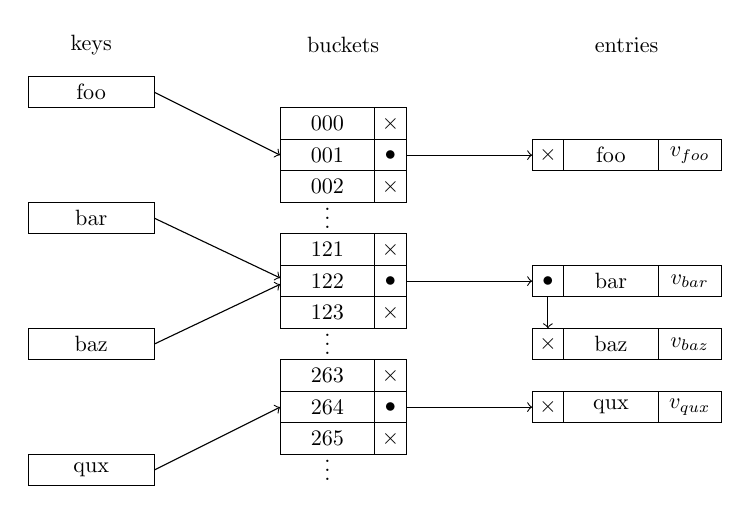
\begin{tikzpicture}[scale=0.8, every node/.style ={scale=0.8}]
        \node at (1,7) {keys};
        \node at (5,7) {buckets};
        \node at (9.5,7) {entries};
        \draw % keys
            (0,6) rectangle node {foo} (2,6.5)
            (0,4) rectangle node {bar} (2,4.5)
            (0,2) rectangle node {baz} (2,2.5)
            (0,0) rectangle node {qux} (2,0.5);
        \draw % buckets, left side
            (4,5.5) rectangle node {$000$} (5.5,6)
            (4,5.0) rectangle node {$001$} (5.5,5.5)
            (4,4.5) rectangle node {$002$} (5.5,5)
            (4.75,4.35) node {$\vdots$}
            (4,3.5) rectangle node {$121$} (5.5,4)
            (4,3) rectangle node {$122$} (5.5,3.5)
            (4,2.5) rectangle node {$123$} (5.5,3)
            (4.75,2.35) node {$\vdots$}
            (4,1.5) rectangle node {$263$} (5.5,2)
            (4,1) rectangle node {$264$} (5.5,1.5)
            (4,0.5) rectangle node {$265$} (5.5,1)
            (4.75,0.35) node {$\vdots$};
        \draw % buckets, right side
    		\foreach \i in {0,1,2} {
    			\foreach \j in {0,2} {
    				(5.5,5.5-2*\i-0.5*\j) rectangle node {$\times$} (6,6-2*\i-0.5*\j)
    			}
    		}
    		\foreach \i in {0,1,2} {
    			(5.5,5.5-2*\i-0.5) rectangle node {$\bullet$} (6,6-2*\i-0.5)
    		};
    	\draw % entries, middle side
    		(8.5,5) rectangle node {foo} (10,5.5)
    		(8.5,3) rectangle node {bar} (10,3.5)
    		(8.5,2) rectangle node {baz} (10,2.5)
    		(8.5,1) rectangle node {qux} (10,1.5);
    	\draw % entries, left side
    		(8,5) rectangle node {$\times$} (8.5,5.5)
    		(8,3) rectangle node {$\bullet$} (8.5,3.5)
    		(8,2) rectangle node {$\times$} (8.5,2.5)
    		(8,1) rectangle node {$\times$} (8.5,1.5);
    	\draw % entries, right side
    		(10,5) rectangle node {$v_{\text{foo}}$} (11,5.5)
    		(10,3) rectangle node {$v_{\text{bar}}$} (11,3.5)
    		(10,2) rectangle node {$v_{\text{baz}}$} (11,2.5)
    		(10,1) rectangle node {$v_{\text{qux}}$} (11,1.5);
    		
    	% arrows
    	\draw[->] (2,6.25) -- (4,5.25);
    	\draw[->] (2,4.25) -- (4,3.30);
    	\draw[->] (2,2.25) -- (4,3.20);
    	\draw[->] (2,0.25) -- (4,1.25);
    	\draw[->] (6,5.25) -- (8,5.25);
    	\draw[->] (6,3.25) -- (8,3.25);
    	\draw[->] (8.25,3) -- (8.25,2.5);
    	\draw[->] (6,1.25) -- (8,1.25);
    \end{tikzpicture}
    \caption{Hash collision resolved by separate chaining.}
    \label{fig:separate_chaining}
\end{figure}

\begin{example}
    Say we have a hash table with hash function $h$ that implements separate chaining for collision resolution. Suppose we add the keys foo, bar, baz, and qux (in the order given) where $h(\text{foo})=001$, $h(\text{bar})=122$, $h(\text{baz})=122$, and $h(\text{qux})=264$. As the keys bar and baz collide, the list at $122$ will contain the first key, bar, and the second key, baz, along with their respective values. The hash table for this example can be found in Figure \ref{fig:separate_chaining}
\end{example}

\begin{definition}
    In \textbf{linear probing}, if we try and insert an entry $(k,v)$ into a bucket $A[i]$ that is already occupied, where $i=h(k)$, then we try next at $A[i+1\bmod N]$. If $A[i+1\bmod N]$ is occupied, then we try $A[i+2\bmod N]$, and so on, until we find an empty bucket that can accept the entry.
\end{definition}

\begin{figure}
    \centering
    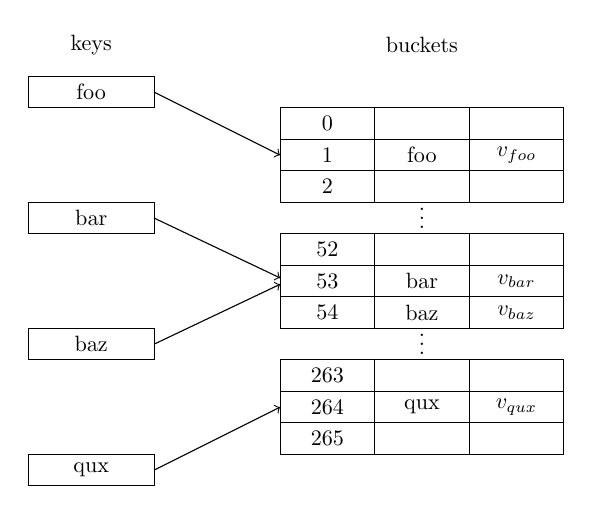
\begin{tikzpicture}[scale=0.8, every node/.style ={scale=0.8}]
        \node at (1,7) {keys};
        \node at (6.25,7) {buckets};
        \draw % keys
            (0,6) rectangle node {foo} (2,6.5)
            (0,4) rectangle node {bar} (2,4.5)
            (0,2) rectangle node {baz} (2,2.5)
            (0,0) rectangle node {qux} (2,0.5);
        \draw % buckets, left side
            (4,5.5) rectangle node {$0$} (5.5,6)
            (4,5) rectangle node {$1$} (5.5,5.5)
            (4,4.5) rectangle node {$2$} (5.5,5)
            (6.25,4.35) node {$\vdots$}
            (4,3.5) rectangle node {$52$} (5.5,4)
            (4,3) rectangle node {$53$} (5.5,3.5)
            (4,2.5) rectangle node {$54$} (5.5,3)
            (6.25,2.35) node {$\vdots$}
            (4,1.5) rectangle node {$263$} (5.5,2)
            (4,1) rectangle node {$264$} (5.5,1.5)
            (4,0.5) rectangle node {$265$} (5.5,1);
    	\draw % buckets, right side
    		\foreach \i in {0,1,2}{
    			\foreach \j in {0,1,2}{
    				(5.5,5.5-2*\i-0.5*\j) rectangle (7,6-2*\i-0.5*\j)
    				(7,5.5-2*\i-0.5*\j) rectangle (8.5,6-2*\i-0.5*\j)
    			}
    		}
    		(6.25,5.25) node {foo}
    		(6.25,3.25) node {bar}
    		(6.25,2.75) node {baz}
    		(6.25,1.25) node {qux}
    		(7.75,5.25) node {$v_{\text{foo}}$}
    		(7.75,3.25) node {$v_{\text{bar}}$}
    		(7.75,2.75) node {$v_{\text{baz}}$}
    		(7.75,1.25) node {$v_{\text{qux}}$};
    		
    	% arrows
    	\draw[->] (2,6.25) -- (4,5.25);
    	\draw[->] (2,4.25) -- (4,3.3);
    	\draw[->] (2,2.25) -- (4,3.2);
    	\draw[->] (2,0.25) -- (4,1.25);
    \end{tikzpicture}
    \caption{Hash collision resolve by linear probing.}
    \label{fig:linear_probing}
\end{figure}

\begin{example}
    Suppose we have a hash table with hash function $h$ that implements linear probing for collision resolution. Suppose we add the keys foo, bar, baz, and qux (in that order) where $h(\text{foo})=1$, $h(\text{bar})=53$, $h(\text{baz})=53$, and $h(\text{foo})=264$. Then we would get foo stored at index $1$, bar stored at index $53$, baz stored at index $54$, and qux stored at $264$. The hash table for this example can be found in Figure \ref{fig:linear_probing}. 
\end{example}

\begin{definition}
    In \textbf{quadratic probing}, we iteratively try the buckets \[A[(i+f(j))\bmod N]\qquad\;\forall\;j\in\mathbb Z_{\geq0}\text{ where }f(j)=j^2.\] This method avoids clustering patterns that occur with linear probing.
\end{definition}

\begin{definition}
    In \textbf{double hashing}, we have two hash functions: $h$ and $h'$. We have that function $h$ maps some key $k$ to a bucket $A[i]$, with $i=h(k)$. If the bucket is already occupied, then we iteratively try the buckets $A[(i+jh'(k))\bmod N]$ for $j=0,1,2,\ldots$.
\end{definition}
